\documentclass{standalone}
\usepackage{tikz}

\begin{document}

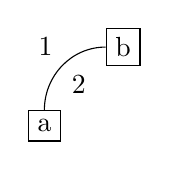
\begin{tikzpicture}
%x description="draw a line with a corner using absolute coordinates"

\node[draw] (a) at (0,0) {a};
\node[draw] (b) at (1,1) {b};

%x step={
\draw (a) 
	to [out=90, in=180] 
	node [auto] {1}
	% swap 'mirrors' the node position
	node [auto, swap] {2}
	(b);
%x }
\end{tikzpicture}

\end{document}
